\section{Bisimulation algorithm (probably in the background section...)}

\newcommand{\nBlue}{\mathit{blue}\xspace}
\newcommand{\nGreen}{\mathit{green}\xspace}
\newcommand{\nSmall}{\mathit{small}\xspace}
\newcommand{\nBig}{\mathit{big}\xspace}
\newcommand{\nBall}{\mathit{ball}\xspace}
\newcommand{\nCube}{\mathit{cube}\xspace}
\newcommand{\nOntop}{\mathit{ontop}\xspace}
\newcommand{\nTop}{\mathit{top}\xspace}
\newcommand{\nBelow}{\mathit{below}\xspace}
\newcommand{\nRightof}{\mathit{rightof}\xspace}
\newcommand{\nLeftof}{\mathit{leftof}\xspace}
\newcommand{\nLeft}{\mathit{left}\xspace}


Refinement algorithms for GRE are based on the following basic idea: given a 
scene $S$, the objects appearing in $S$ are successively classified according
to their properties into finer and finer classes. A description (in some formal language $\mathcal{L}$)  of each 
class is computed every time a class is refined. The procedure always stops when the 
set of classes stabilizes, i.e., no further refinement is possible with the information 
available in the scene\footnote{Of course, if we are only interested in a referring expression for 
a given target we can stop the procedure as soon as the target is the only element of some of the classes.}.
If the target element is in a singleton class, then 
the formal description of that class is a referring expression; otherwise the 
target cannot be unequivocally described (in $\mathcal{L}$).  

It is clear that a scene can be encoded in different ways as a relational model (for example in \ref{figure22}, we could argue that $e_1$ is also \emph{leftof} $e_2$, not considered because they are no touching).  The algorithm assumes that these issues have been resolved and that the model encodes a suitable representation of the scene we want to describe.  Moreover, we will assume that all relations are \emph{binary}.  We will not consider relations of arity greater than two (relations of higher arity can be encoded as binary relations via reification, if necessary).

On termination, the algorithm computes what are called the $\mathcal{L}$-similarity classes of the input model $\gM$. Intuitively, the referring expression ``$ball$'' and ``$cube$''  are more specific and then contain more information than $\top$.

%There is many $\mathcal{L}$, we will name $\alc$ and $\el$

ACA VOY A PONER gramatica para generar... ALC y EL

In what follows, we use formulas of the $\el$ description logic language~\cite{baad:desc03} to describe refinement classes \footnote{Notice, though, that the particular formal language used is independent of the main algorithm, and different add$_{\mathcal{L}}$(R,$\varphi$,\RE) functions can be used depending on the language involved.}.
 As discussed in~\cite{arec2:2008:Areces}, this language is suitable for describing conjunctive and relational REs, which are the ones we find in  corpora. 

The input to the algorithm will be a relational model $\mathcal{M} = \tup{\Delta, \interp{\cdot}}$,
where $\Delta$ is the non-empty domain of objects in the scene, and $\interp{\cdot}$ is an 
interpretation function that assigns to all properties in the scene their intended extension.  For example, 
the scene shown in Figure~\ref{GRE3D7-stimulus} could be represented by the model $\gM=\tup{\Delta,\interp{\cdot}}$ shown in Figure~\ref{GRE3D7-stimulus-graph}; where $\Delta = \{e_1,\ldots,e_7\}$, and $\interp{\emph{green}}$ is $\{e_3,e_4,e_6\}$.

$\top$ is a formula that represents the most general description whose interpretation includes all elements of the model. It could be realize as the RE with the noun ``thing''. We say that a formula is \emph{subsumed} by other formulas, if it extension can be cover by the union of the extensions of the other formulas. For example, in Figure~\ref{figure22}, $\top$ is subsumed by ball and cube, because $\interp{\top}$ = $\interp{ball} \cup \interp{cube}$ = $\{e_2, e_4, e_6, e_7\}$, it is $\{e_1, e_2, e_3, e_4, e_5, e_6, e_7\}$ = $\{e_1, e_3, e_5\} \cup \{e_2, e_4, e_6, e_7\}$. Intuitively the formula cube or ball have more information than $\top$, for each element of $\top$, there is a formula that gives more information, say ``cube'' is more informative than say ``thing''.\\

In the following we will explain an example of execusion of the algorithm shown in ~\ref{algoritmoOriginal} taking into account the $\el$ logic language. This algorithm where first presented in~\cite{arec2:2008:Areces}.
\begin{figure}[h!]
\begin{center}
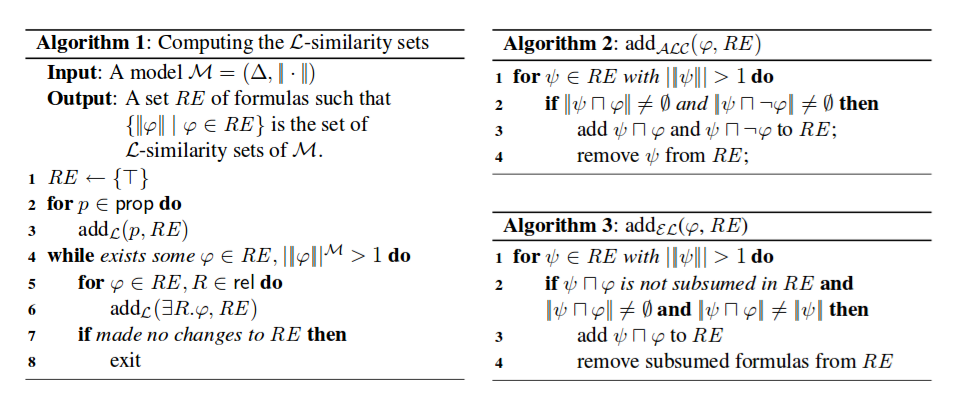
\includegraphics[width=\textwidth]{images/algoritmoOriginal.png}
\end{center}
\vspace*{-2em}
\caption{Algorithms}
\label{Algorithms }
\end{figure}

\subsection{An example of execusion}

We will run the algorithm for the Scene~\ref{figure22}, the algorithm start with a fixed list of properties and relations, supose that those lists are the following:

ordered properties (prop): ball, cube, red, yellow, small, large.\\
ordered relations (rel): leftof, rightof, ontopof, bellowof.

\begin{figure}
\begin{center}
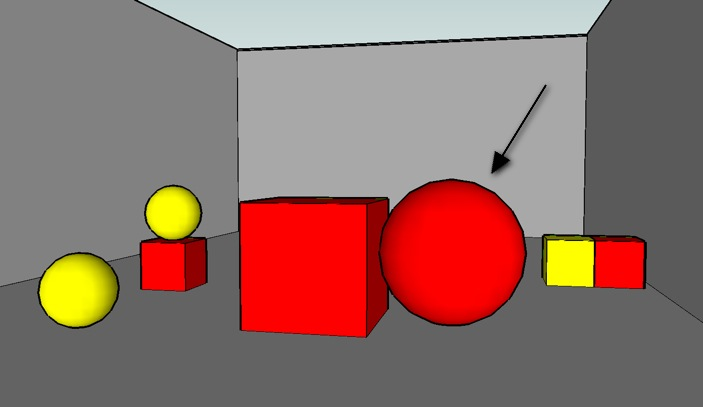
\includegraphics[width=.5\textwidth]{images/22.jpg}
\end{center}
\vspace*{-2em}
\caption{A 3D scene of geometric figures}
\label{figure22}
\end{figure}

We will return RE, there will be a formula for each element in the domain (if that formula exists or that model).\\

In the begining RE=$\{\top\}$ and its $\interp{\top}$ = $\{e_1, e_2, e_3, e_4, e_5, e_6, e_7\}$\\

The first loop for of the algorithm is in the properties. For each property realize add$\el$ ($\varphi$, RE),

A formula $\varphi$ will be added to RE if its interpretation has at least one element, then for each formula $\psi$ in RE the conjunction 
$\varphi  \cup \psi$ need to be not subsumed in RE, the $\interp{\varphi \cup \psi}$ need to be not empty, and its interpretation need to be distinct of $\interp{\psi}$ as we can see in the algorithm~\ref{algoritmoOriginal}.

So first we add the formula \textsf{ball}, so RE = \{$\top$, ball\} then the formula ``cube'', so RE = \{$\top$, ball, cube\}, now we have that $\interp{ball}$ = $\{e_1, e_3, e_5\}$, $\interp{cube}$ = $\{e_2, e_4, e_6, e_7\}$, so, we are capable to delete $\top$, because it is subsumed to the two other sets. The turn is now for the formula ``red'', $\interp{red}$ is: $\{e_2, e_4, e_5, e_7\}$, doing the intersection with the $\interp{.}$ of each formula in RE we obtain, $\{e_5\}$ and $\{e_2, e_4, e_7\}$, now RE = $\{ball, cube, ball \wedge red, cube \wedge red\}$, following with ``yellow'', we have, $\interp{yellow}$ = $\{e_1, e_3, e_6\}$ and we obtain RE = $\{ball \wedge yellow, cube \wedge yellow, ball \wedge red, cube \wedge red\}$ note than here we already delete the formula ``ball'' because it was subsumed, and the formula ``cube'' too.
Doing the same with ``small'' we have RE = $\{ball \wedge yellow \wedge small, cube \wedge yellow \wedge small, ball \wedge red, cube \wedge red, cube \wedge red \wedge small\}$. Next property is ``large'' so, we have RE = $\{ball \wedge yellow \wedge small, cube \wedge yellow \wedge small, ball \wedge red, cube \wedge red \wedge large, cube \wedge red \wedge small\}$. Note that here we cannot add ``large'' to a formula ``$red \wedge cube$'' because it interpretation has only one element, and the condition say that it need to have more than one in order to add the intersection with others formulas.

Until now RE = $\{ball \wedge yellow \wedge small, cube \wedge yellow \wedge small, ball \wedge red, cube \wedge red \wedge large, cube \wedge red \wedge small\}$ and we have the following extensions: $\{e_1, e_3\}, \{e_6\}, \{e_5\}, \{e_4\}, \{e_2, e_7\}$. There is two formulas that can be refined more, the  $ball \wedge yellow \wedge small$ and $cube \wedge red \wedge small$ because they have more than one element each, so we enter en in the while cicle of Algorithm 1, in line 4. Now is the turn of relations, the first one is ``leftof'' we for each formula $\varphi$ in RE will try to add$\el$ ($\exists leftof.\varphi$, RE). Note that $\psi$ only can be $ball \wedge yellow \wedge small$ or  $cube \wedge red \wedge small$ because those are the ones that its interpretation have more than one element. There is not $\varphi$ and $\psi$ that can be apply. Continuing with rightof we add $cube \wedge yellow \wedge small \wedge \exists rightof. cube \wedge red \wedge small$, and so on with ``topof'' we add $small \wedge red \wedge cube \wedge \exists ontop. small \wedge yellow \wedge ball$ and the algoritm ends with RE = $\{ball \wedge yellow \wedge small, cube \wedge yellow \wedge small, ball \wedge red, cube \wedge red \wedge large, cube \wedge red \wedge small, cube \wedge yellow \wedge small \wedge \exists rightof. cube \wedge red \wedge small, small \wedge red \wedge cube \wedge \exists ontop. small \wedge yellow \wedge ball\}$, here all elements are in a singleton class and not further refinement can be done.


%can be applied to $cube \wedge red \wedge small$ but there is no formula which interpretation has more than one element to be apply with this one. The same happen for the other relations, so the algorithm ends.
%its interpretation is $\{e_7\}$ with $\psi$ is $cube \wedge yellow \wedge small$, the others combinations can't be apply because they don't do true the preconditions. The following relation is rightof, 

%leftof, rightof, ontopof, bellowof

%At this point we already have the target in a singleton set. So the formula for it is ``red and ball'', and also for s6 which formula is ``yellow cube''.\\
%As we show this algorithm depends of the order of properties and relations.\\

\section{Adding probabilities to a symbolic algorithm} \label{sec:algorithm}

In this section we present a modification of the algorithm in~\cite{arec2:2008:Areces} where the fixed order of the properties in the 
input scene is replaced by a finite probability distribution.  The required changes
are fairly straightforward (see Figures~\ref{fig:algo1} and~\ref{fig:algo2}), but 
the behavior of the resulting algorithm is strikingly changed. To start with, the 
algorithm is now non-deterministic: two runs of the algorithm with the same 
input might result in different REs for the objects in the scene.  Putting 
it differently, we can now generate a distribution probability for the REs generated by the algorithm by repeatedly running 
it over the same input.  As we will empirically show in Section~\ref{sec:evaluation}, given a 
corpus of REs for a given scene, it is possible to compute a suitable probability 
distribution for the probability of use of the relations in the scene, in such a way that the probability 
distribution of the REs generated by the model simulates the one found in the corpus.

We consider unary
properties encoded as binary relations including one additional `dummy' element in the model (e.g., we encode the fact that $e_1$ is \emph{blue} saying that it is related to the dummy element by the \emph{blue} binary relation).

%In order to understand how the algorithm works, and the differences with the original proposal, {\it MOVED we need first to introduce some 
%basic notions.  The input to the algorithm will be a relational model $\mathcal{M} = \tup{\Delta, \interp{\cdot}}$,
%where $\Delta$ is the non-empty domain of objects in the scene, and $\interp{\cdot}$ is an 
%interpretation function that assigns to all properties in the scene its intended extension.  For example, 
%the scene shown in Figure~\ref{GRE3D7-stimulus} could be represented by the model $\gM=\tup{\Delta,\interp{\cdot}}$ shown in Figure~\ref{GRE3D7-stimulus-graph}; where $\Delta = \{e_1,\ldots,e_7\}$, and $\interp{\emph{green}}$, for example, is $\{e_3,e_4,e_6\}$.}


\begin{figure}[ht]
\begin{minipage}[b]{0.45\linewidth}
\centering
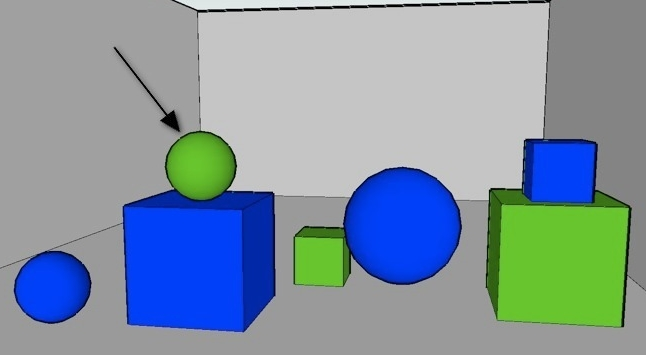
\includegraphics[width=\textwidth]{images/3.jpg}
\vspace*{.15cm}
%\caption{Input scene}
\label{GRE3D7-stimulus}
\end{minipage}
\hspace*{-0.35cm}
\begin{minipage}[b]{0.6\linewidth}
\centering
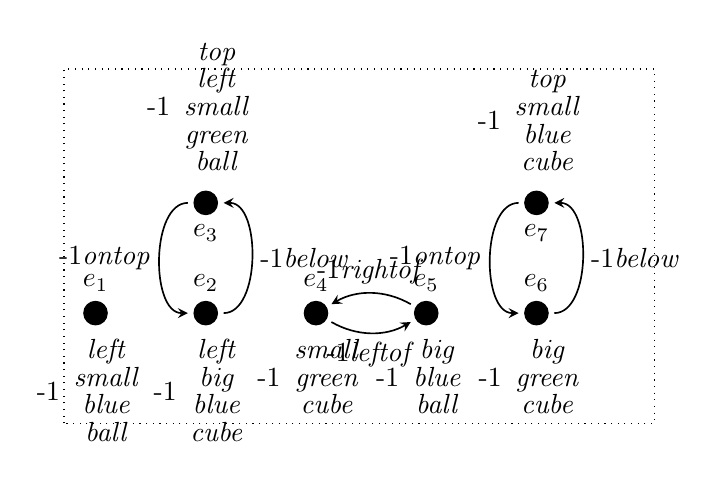
\begin{tikzpicture}
  [
    n/.style={circle,fill,draw,inner sep=3pt,node distance=1.4cm},
    aArrow/.style={->, >=stealth, semithick, shorten <= 2pt, shorten >= 2pt},
  ]
 \node[n,label=above:$e_1$,label=below:{
    \relsize{-1}$\begin{array}{c}
      \nLeft\\[-2pt]
      \nSmall\\[-2pt] 
      \nBlue \\[-2pt] 
      \nBall\end{array}$}] (a) {};

 \node[n,label=above:$e_2$,label=below:{
    \relsize{-1}$\begin{array}{c}
      \nLeft\\[-2pt]
      \nBig\\[-2pt] 
      \nBlue\\[-2pt] 
      \nCube\end{array}$}, right of=a] (b) {};

 \node[n,label=below:$e_3$,label=above:{
    \relsize{-1}$\begin{array}{c}
      \nTop\\[-2pt]
      \nLeft\\[-2pt]
      \nSmall\\[-2pt] 
      \nGreen\\[-2pt] 
      \nBall\end{array}$}, above of=b] (c) {};

 \node[n,label=above:$e_4$,label=below:{
    \relsize{-1}$\begin{array}{c}
      \nSmall\\[-2pt] 
      \nGreen\\[-2pt] 
      \nCube\end{array}$}, right of=b] (d) {};

 \node[n,label=above:$e_5$,label=below:{
    \relsize{-1}$\begin{array}{c}
      \nBig\\[-2pt] 
      \nBlue\\[-2pt] 
      \nBall\end{array}$}, right of=d] (e) {};

 \node[n,label=above:$e_6$,label=below:{
    \relsize{-1}$\begin{array}{c}
      \nBig\\[-2pt] 
      \nGreen\\[-2pt] 
      \nCube\end{array}$}, right of=e] (f) {};

 \node[n,label=below:$e_7$,label=above:{
    \relsize{-1}$\begin{array}{c}
      \nTop\\[-2pt]
      \nSmall\\[-2pt] 
      \nBlue\\[-2pt] 
      \nCube\end{array}$}, above of=f] (g) {};

 \draw [aArrow,bend right=90] (b) to node[auto,swap]{\relsize{-1}$\nBelow$} (c);
 \draw [aArrow,bend right=90] (c) to node[auto,swap]{\relsize{-1}$\nOntop$} (b);

 \draw [aArrow,bend right=30] (d) to node[auto,swap]{\relsize{-1}$\nLeftof$} (e);
 \draw [aArrow,bend right=30] (e) to node[auto,swap]{\relsize{-1}$\nRightof$} (d);

 \draw [aArrow,bend right=90] (f) to node[auto,swap]{\relsize{-1}$\nBelow$} (g);
 \draw [aArrow,bend right=90] (g) to node[auto,swap]{\relsize{-1}$\nOntop$} (f);

 \draw[dotted] (-.4,-1.4) rectangle (7.1,3.1);

 \end{tikzpicture}
\caption{Scene as a relational model}
\label{GRE3D7-stimulus-graph}
\end{minipage}
\end{figure}

%It is clear that a scene can be encoded in different ways as a relational model (for example, we could argue that $e_1$ is also \emph{leftof} $e_2$, and so on).  The algorithm assumes that these issues have been resolved and that the model encodes a suitable representation of the scene we want to describe.  Moreover, we will assume that all relations are \emph{binary}.  We will not consider relations of arity greater than two (relations of higher arity can be encoded as binary relations via reification, if necessary), and unary
%properties can be encoded as binary relations including one additional `dummy' element in the model (e.g., we encode the fact that $e_1$ is \emph{blue} saying that it is related to the dummy element by the \emph{blue} binary relation).

%On termination, the algorithm computes what are called the $\mathcal{L}$-similarity classes of the input model $\gM$. Intuitively, if two elements in the model belong to the same $\mathcal{L}$-similarity class, then $\mathcal{L}$ is not expressive enough to tell them appart (i.e, no formula in $\mathcal{L}$ can distinguish them). 

%In what follows, we will use formulas of the $\el$ description logic language~\cite{baad:desc03} to describe refinement classes.  As discussed in~\cite{arec2:2008:Areces}, this language is suitable for conjunctive relational RE, which are the ones we will find in the corpora used for our evaluation\footnote{Notice, though, that the particular formal language used is independent of the main algorithm, and different add$_{\mathcal{L}}$(R,$\varphi$,\RE) functions can be used depending on the language involved.}. For a detail description of $\el$, we refer to~\cite{baad:desc03}.  For this paper, we only need to know that the interpretation of the formula $\psi \sqcap \exists$R.$\varphi$ is the set of all elements that satisfy $\psi$ and that are related by relation R to some element that satisfy $\varphi$. For example, the interpretation of the formula \emph{ball} $\sqcap \exists$\emph{leftof}.\emph{cube} is the set of all balls that are on the left of some cube.  

We are now ready to describe Algorithms~\ref{algo:bisim-l} and~\ref{algo:bisim-add-el}. Algorithm~\ref{algo:bisim-l} takes as input a model $\gM$ and a list Rs of pairs (R,R.\puse) that links each relation R to some probability of use R.\puse. I.e., if $\REL$ is the set of all relation symbols in the model (i.e., the \emph{signature} of the model) then Rs $\in (\REL \times [0,1])^*$. Moreover, we assume Rs to be ordered by R.\puse. 

\begin{figure}[t]
\small
\centering
\begin{algorithm}[H]
\dontprintsemicolon
\caption{Computing $\mathcal{L}$-similarity classes}\label{algo:bisim-l}
\KwIn{\footnotesize A model $\gM$ and a list Rs $\in (\REL \times [0,1])^*$
 of relation symbols with their \puse\ values, ordered by \puse}
\KwOut{\footnotesize A set of formulas \RE such that
$\{\interp{\varphi} \mid \varphi \in \RE\}$ is the set of
$\mathcal{L}$-similarity classes of $\gM$}

$\RE \leftarrow \{\top\}$\tcp*[f]{\footnotesize the most general description $\top$ applies to all elements in the scene}

\For{\em (R,R.\puse) $\in$ Rs}{
	R.\randomuse = Random(0,1)\tcp*[f]{\footnotesize R.\randomuse is the probability of using R} \;
        R.\incuse = (1 $-$ R.\puse) / MaxIterations\tcp*[f]{\footnotesize R.\puse\ are incremented by R.\incuse in each loop}
}

\Repeat{\em $\forall$((R,R.\puse) $\in$ Rs).(R.\puse $\ge$ 1)\tcp*[f]{\footnotesize R.\puse\ are incremented until they reach 1}}{
  \While(\tcp*[f]{\footnotesize while some class has at least two elements}){\em $\exists (\varphi \in$ \RE)$.(|\interp{\varphi}|>1)$}{
      \RE' $\leftarrow$ \RE \tcp*[f]{\footnotesize make a copy for future comparison} \;
      \For{\em (R, R.\puse) $\in$ Rs}{
          \If(\tcp*[f]{\footnotesize R will be used in the expression}){\em R.\randomuse $\le$ R.\puse}{
              \For{\em $\varphi \in$ \RE}{
                  add$_\mathcal{L}$(R, $\varphi$, \RE)\tcp*[f]{\footnotesize refine all classes using R}}
                  }\;
              \If(\tcp*[f]{\footnotesize the classification has changed}){\em \RE $\not =$ \RE'}{exit\tcp*[f]{\footnotesize exit for-loop to try again highest R.\puse}}
              }
     \If(\tcp*[f]{\footnotesize the classification has stabilized}){\em \RE $=$ \RE'}{exit\tcp*[f]{\footnotesize exit while-loop to increase R.\puse}}
  }
  \For{\em (R,R.\puse) $\in$ Rs}{
    R.\puse $\leftarrow$ R.\puse $+$ R.\incuse\tcp*[f]{\footnotesize increase R.\puse}
  }
}
\end{algorithm}
\vspace*{-.5cm}\caption{Main algorithm, dealing with probabilities}\label{fig:algo1}
\end{figure}


\begin{figure}[t]
\small
\centering
\begin{algorithm}[H]
\dontprintsemicolon
\caption{add$_\el$(R, $\varphi$, \RE)} \label{algo:bisim-add-el}

\For{\em $\psi \in$ \RE with $|\interp{\psi}| > 1$}{
  \If(\tcp*[f]{\footnotesize informative: smaller than the original?}){\em $\psi \sqcap \exists$R.$\varphi$ is not subsumed in \RE\ {\bf and} \tcp*[f]{\footnotesize non-redundant: can't be obtained from \RE?}\\
    \em \ \ \ $\interp{\psi \sqcap \exists \mbox{\em R}.\varphi} \neq \emptyset$ {\bf and} \tcp*[f]{\footnotesize non-trivial: has elements?}\\
     \ \ \ $\interp{\psi \sqcap \exists \mbox{\em R}.\varphi} \neq \interp{\psi}$ }{
    add $\psi \sqcap \exists \mbox{R}.\varphi$ to $\RE$ \tcp*[f]{\footnotesize add the new class to the classification} \;
    remove subsumed formulas from $\RE$ \tcp*[f]{\footnotesize remove redundant classes}
  }
}
\end{algorithm}
\vspace*{-.5cm}\caption{Refinement function for the \el-language}\label{fig:algo2}
\end{figure}

The set $\RE$ will contain the formal description of the refinement classes and it is initialized by the most general description $\top$.  
For each R, we first compute R.\randomuse, a random number in [0,1].  If R.\randomuse $\le$ R.\puse\ then we will use R to refine the set of classes.  The value of R.\puse\ will be incremented by $R.\incuse$ in each main loop, to ensure that all relations are, at some point, considered by the algorithm.  This ensures that a referring expression will be found if it exist; but gives higher probability to expressions using relations with a high R.\puse. 
 
While $\RE$ contains descriptions that can be refined (i.e., classes with at least two elements) we will call the refinement function add$_\mathcal{L}$(R,$\varphi$,$\RE$) successively with each relation in Rs. A change in one of the classes, can trigger changes in others. For that reason, if $\RE$ changes, we exit the for-loop to start again with the relations of higher R.\puse. If the after trying to refine the set with all relations in Rs, the set $\RE$ has not changed, the we have reach a stable state (i.e., the classes described in $\RE$ cannot be further refined, using the current R.\puse\ values). We will then increment all the R.\puse\ values and start the procedure again. 

Algorithm~\ref{algo:bisim-add-el} coincides with the one described in~\cite{arec2:2008:Areces}.  It will refine each of the descriptions in $\RE$ using the relation R and the other descriptions already in $\RE$, under certain conditions. The new description should be \emph{non-redundant} (the new  class cannot be obtained as the union of classes already represented in $\RE$), \emph{non-trivial} (the new class is not empty), and 
\emph{informative} (the new class should not coincide with the original class).  If all this conditions are met, the new description is added to $\RE$, and redundant descriptions possible created by the addition of the new description are eliminated.   

Suppose fixed an input model $\gM$ and values for Rs, and fix also some target element $t$.  Assume also that $t$ indeed has an $\el$-referring expression.  Upon termination, Algorithm~\ref{fig:algo1} will compute an $\el$ formula $\varphi$ such that $\interp{\varphi} = \{t\}$, but $\varphi$ might be different in each run of the algorithm (even though $\gM$ and Rs are fixed).  If we repeat this experiment a statistically significant number of times, we can define an estimate of the probability distribution of the REs generated by the algorithm for $t$, given $\gM$ and Rs. In Section~\ref{sec:evaluation} we will show that given a corpus of REs for $\gM$, it is possible to define R.\puse\ values so that this probability distribution matches with good accuracy the probability distribution of REs found in the corpus.  
